Transportation accessibility measurement is a network problem. Any method which seeks to quantify accessibility must define the nodes and edges which comprise the region in question. In the modern world, all nodes are, to a greater or lesser extent, connected. It is often the case that several modes and paths can be nearly equal in cost. Scoping an accessibility analysis can be highly determinative of outcome. Researchers and planners have primarily utilized the concept of transportation accessibility as it applies to routine household behavior and local travel \cite{Handy_2020}. From the personal transportation perspective, access is defined as the ease with which individuals can reach the opportunities they desire subject to land-use, transportation infrastructure, temporal availability, and individual preference. Land-use dynamics determine the spatial distribution of amenities such as jobs and services as well as that of potential customers. Transportation systems determine the edge traversal costs including travel time, effort, and price which impede flows \cite{Geurs_2004}. Temporal availability of opportunities and transportation modes restrict the utility of opportunities and transportation modes. Characteristics such as age, income, and education predict attraction of opportunities and transportation modes of individuals \cite{Miller_2018}. Any transportation accessibility analysis must, thus, be stochastic.


Many of the most heavily populated Places are adjacent with each other or nearly so. The bulk of traffic between these will be local and routine. For the benefit of clarity and brevity these can be merged into super-Places. This is accomplished by the computation of maximally modular communities. First the distances for all pairs are computed. Second an inverse proximity is computed as

\begin{equation}
	\Gamma_{ij} = \exp{\left(\frac{\Phi_d(i,j)}{\epsilon}\right)}
\end{equation}

where $\epsilon$ is a characteristic distance set at 10 km in this case. Solving for maximally modular communities, centroids of the 34 resulting communities are shown in Figure \ref{fig:california_incorporated_communities}.

\begin{figure}[H]
	\centering
	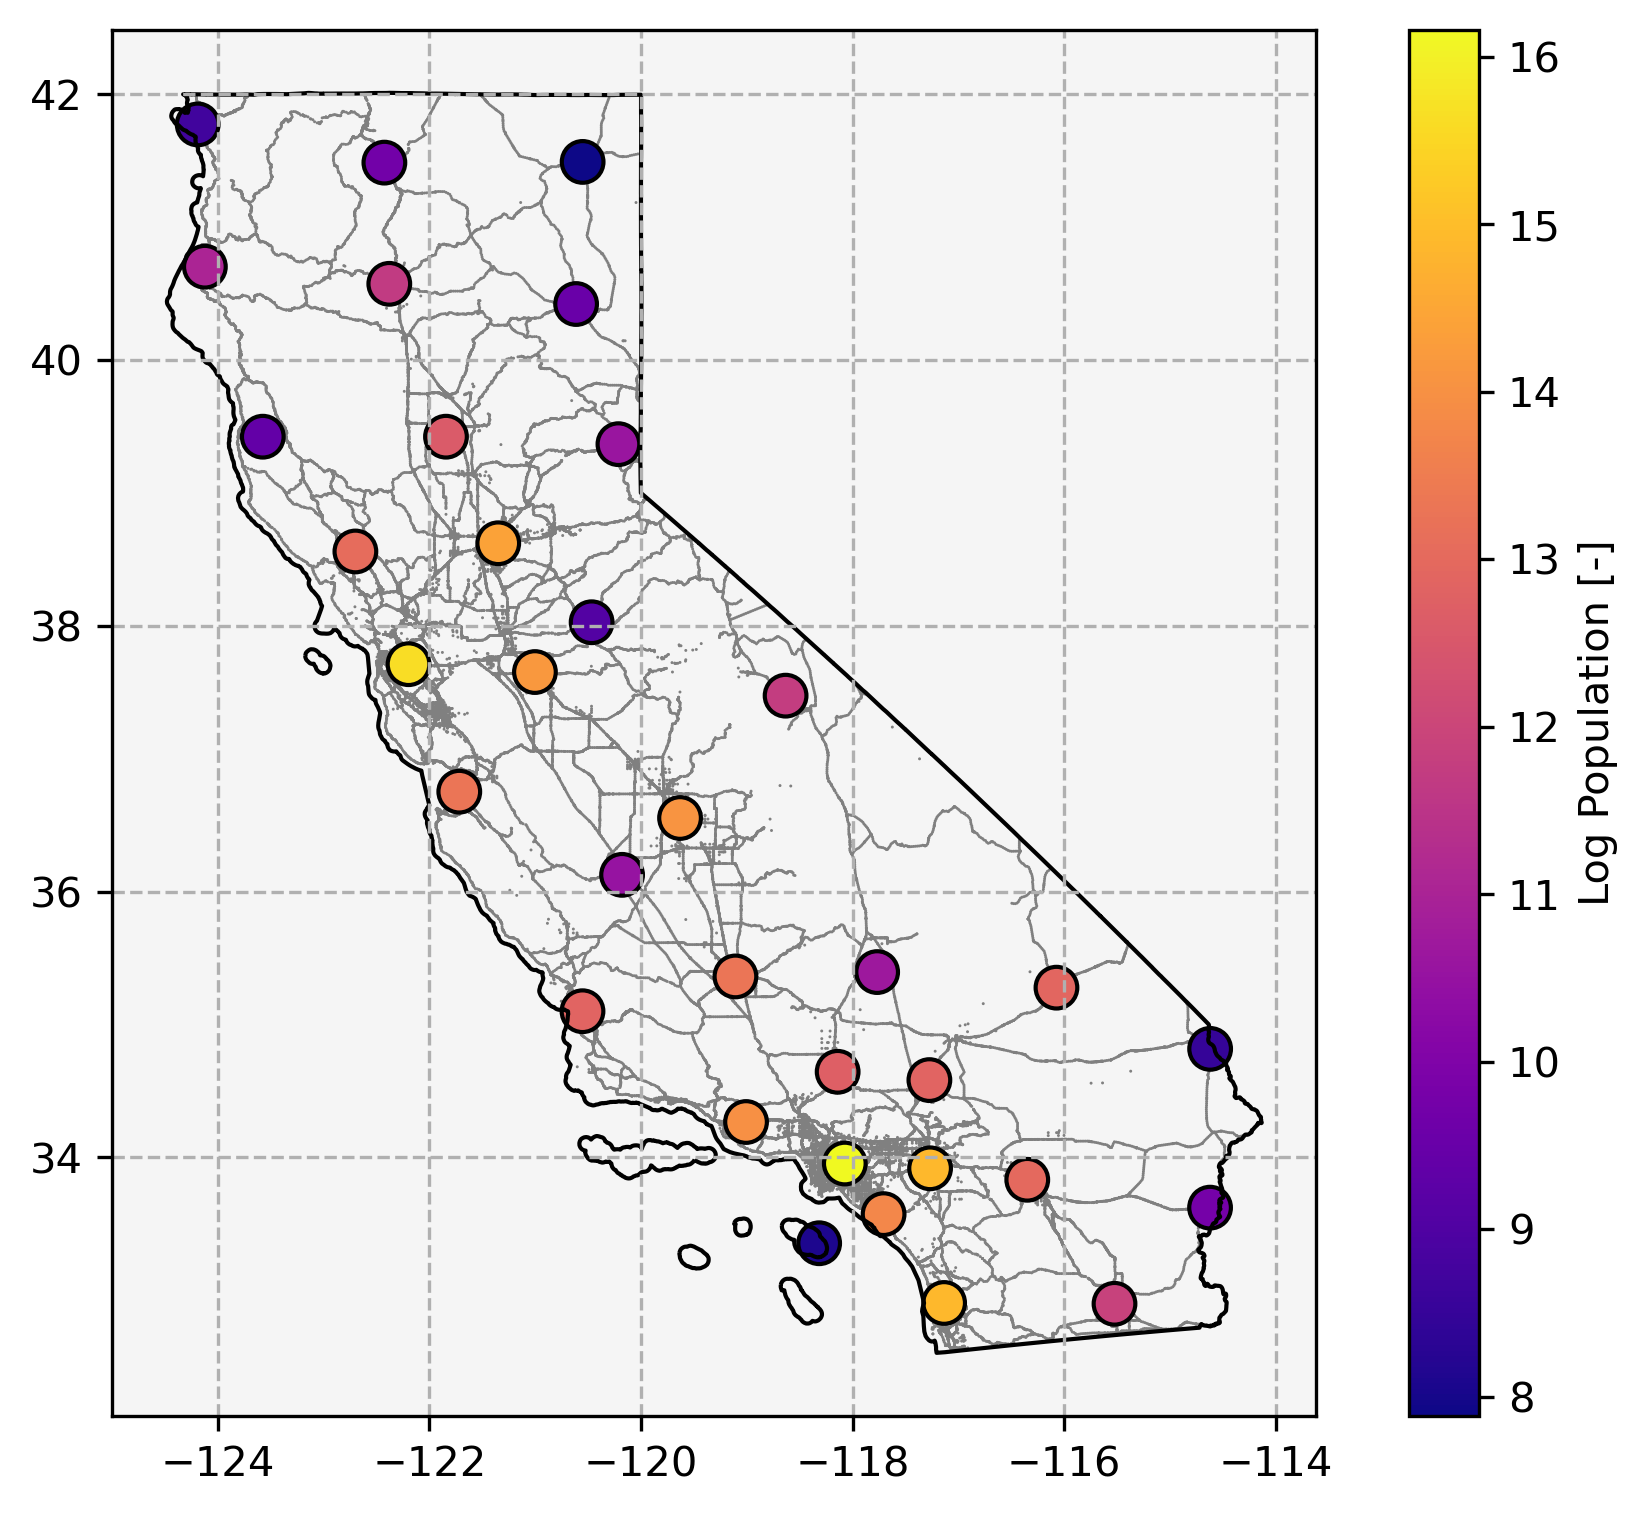
\includegraphics[width = \linewidth]{figs/california_incorporated_communities.png}
	\caption{Natural logarithm  of population for Incorporated Place Communities in California}
	\label{fig:california_incorporated_communities}
\end{figure}

Finally, for the purposes of analysis, points representing departure locations for Phoenix AZ, Las Vegas NV, Reno NV, and Portland/Eugene OR are added to the fringes of the map to represent the associated travel demand.


One way to assess the sufficiency of a vehicle's range is to use the \gls{uf} as defined in SAE J2841 \cite{SAE_J2481}. The \gls{uf} uses \gls{nhts} data \cite{NHTS_2022} to assess the portion of travel that a \gls{phev} can undertake in all-electric mode assuming that every daily itinerary starts at full charge. Figure \ref{fig:utility_factors} shows the \gls{uf} of vehicles by full-charge range with data from the 2022 \gls{nhts}. 

\begin{figure}[H]
	\centering
	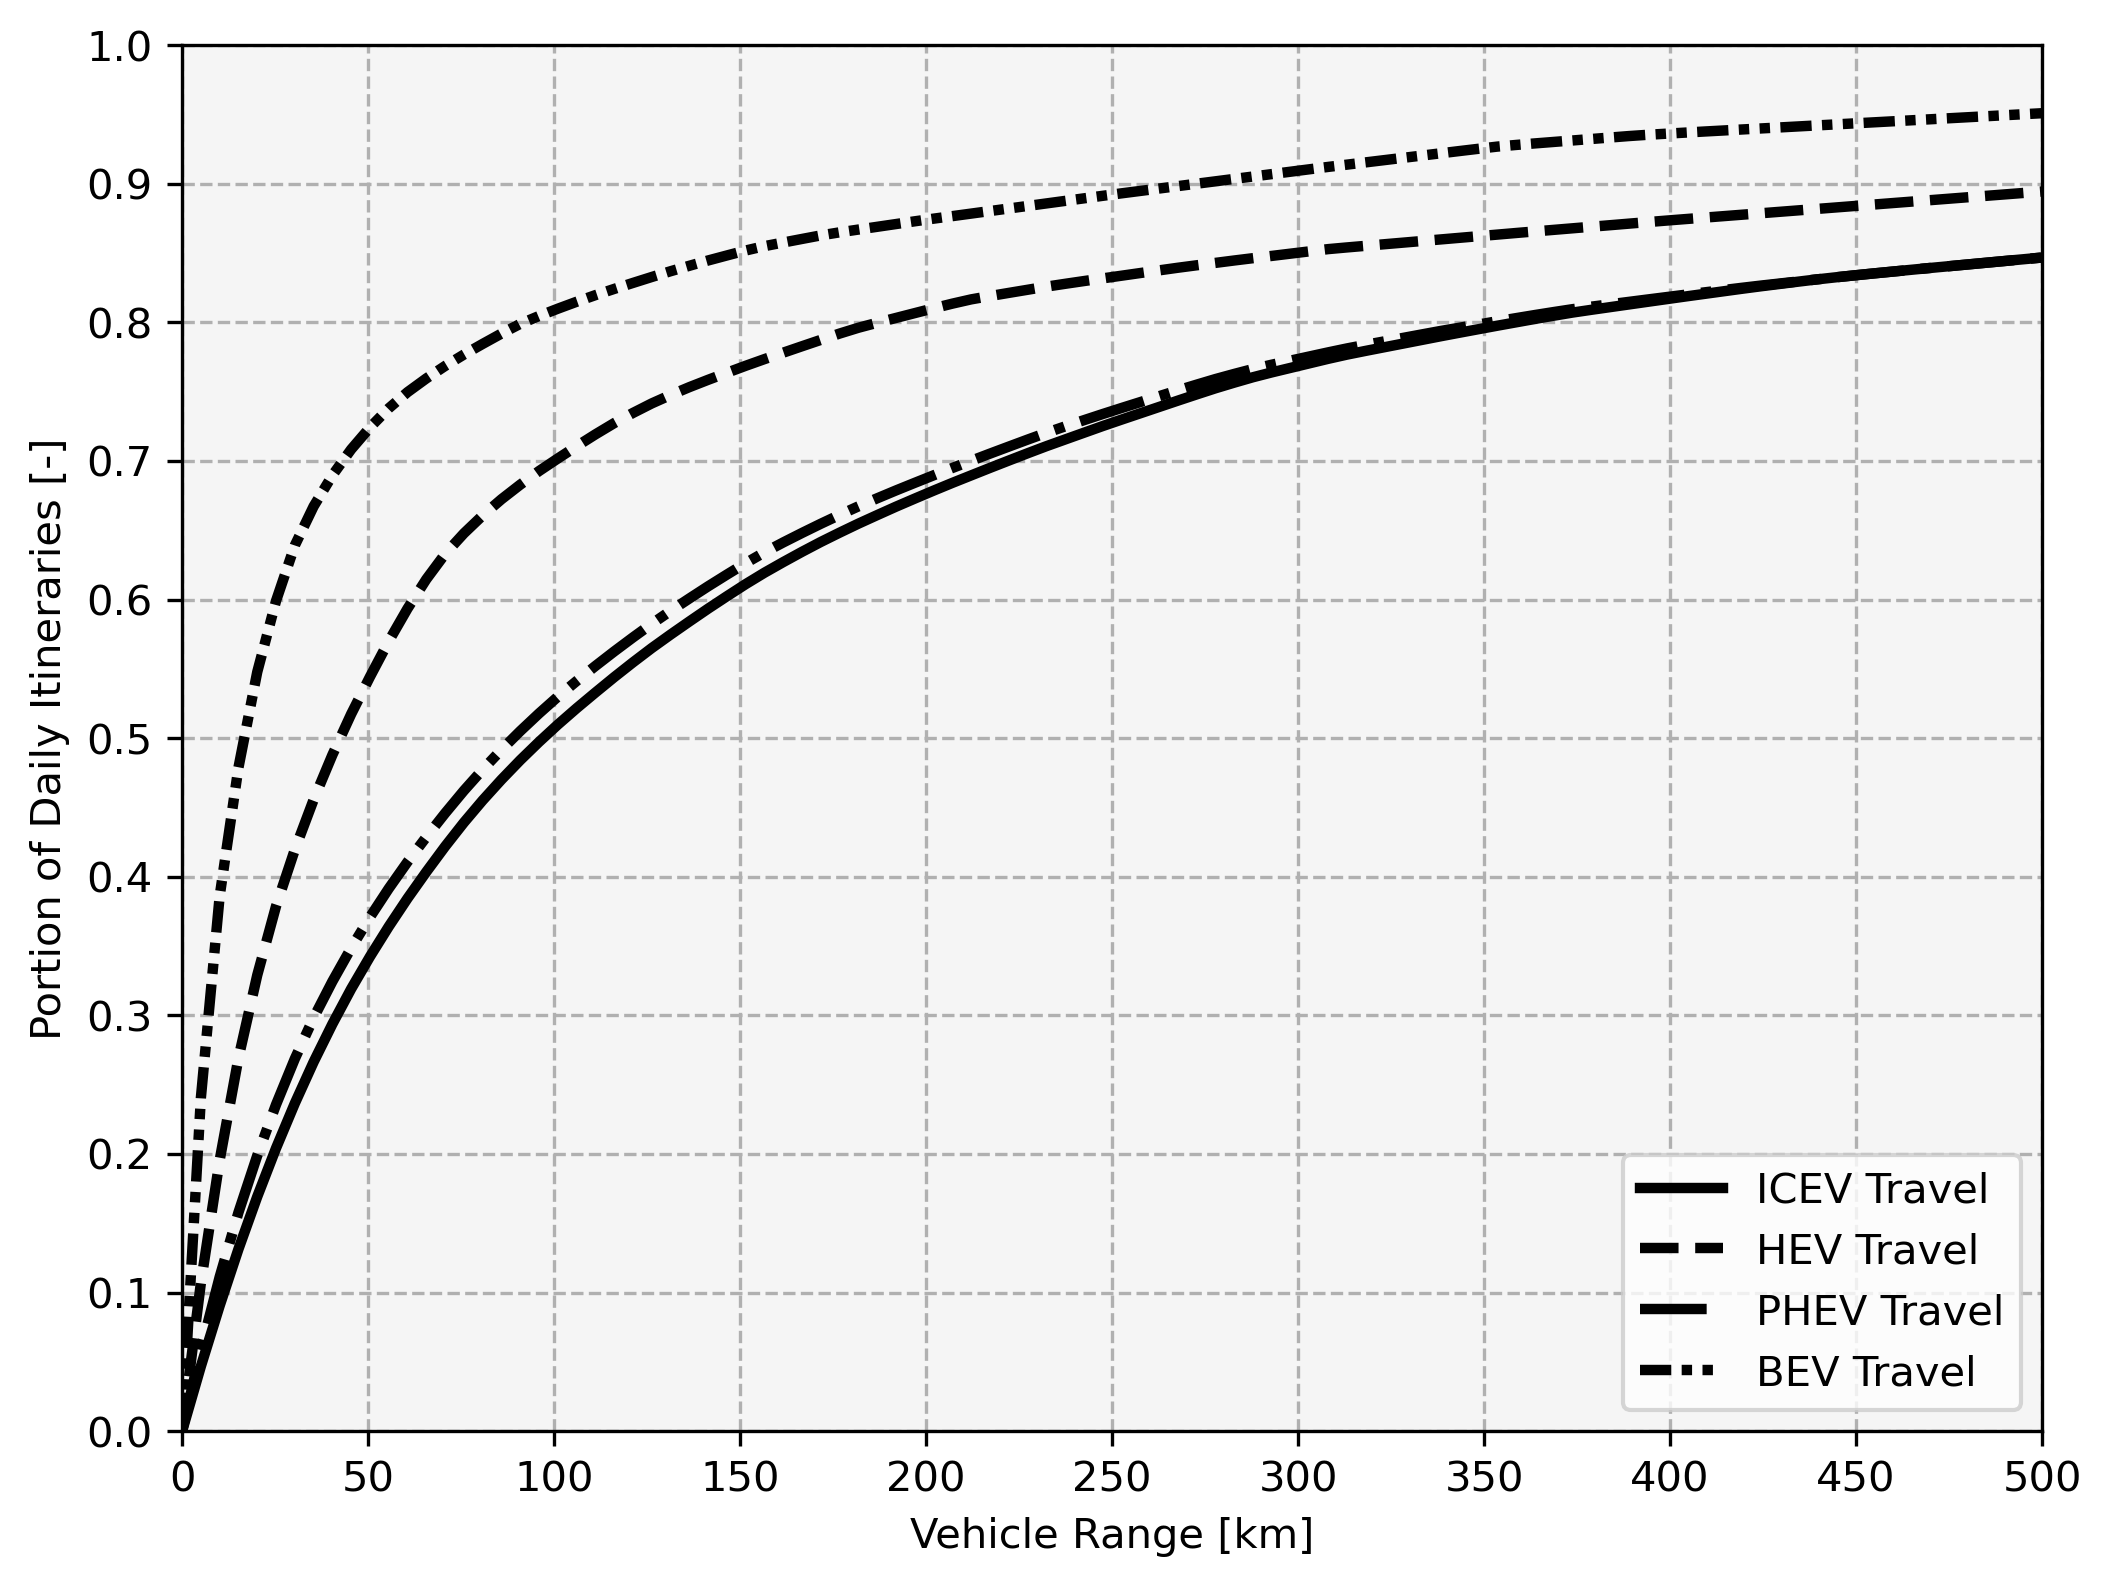
\includegraphics[width = \linewidth]{figs/UF_2022_km.png}
	\caption{Individual vehicle routine travel \glspl{uf} as a function of range by powertrain type for \gls{nhts} 2022 edition}
	\label{fig:utility_factors}
\end{figure}

A takeaway from Figure \ref{fig:utility_factors} is that \glspl{ev} drive shorter daily itineraries. \gls{hev} itineraries are slightly shorter than \gls{icev} but nearly identical. \gls{phev} and \gls{bev} itineraries are substantially shorter than \glspl{icev} itineraries.

Although \glspl{bev} share the roads with \glspl{icev} their operational characteristics (range and charging speeds) and the structure of charging infrastructure dictate that user experience will be different. There is substantial evidence to suggest that a large portion of US drivers consider \gls{bev} capabilities to be a mismatch with their needs.